\section{Scope of the Thesis}

The task of path planning for a robot involves finding an optimal start-to-goal trajectory that enables autonomous intelligent motion. A path planning algorithm for an autonomous robot performs the task of a pilot operating an aircraft, first understanding the environment, then estimating a high-level path from its start to destination and, finally, deciding on the controls necessary to execute this path. It must be aware of the dynamic and hardware constraints associated with the robot mechanical system, while interacting heavily with its environment and adapting its motion to potential changes in its surroundings. The ability of drones, autonomous cars and personal robots to maneuver through complex environments relies on the following components as depicted in Fig \ref{fig:intro_overview_robot}:

\begin{figure}[ht]
    \centering
    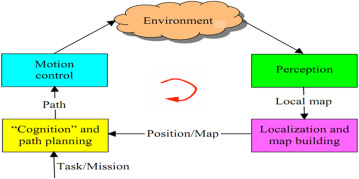
\includegraphics{figures/intro/overview_robot.jpg}
    \caption[Overview of Autonomous Robot Systems]{An overview of the components of an autonomous robot system. The perception component gathers data from the environment and sends a local map to the robot for detecting its own pose, which is eventually sent into the task/path planning module. The planned path or task sequence is finally sent for execution to the low-level motion controller. \textit{Source: \cite{overview_robot}}}
    \label{fig:intro_overview_robot}
\end{figure}

\begin{enumerate}
    \item A data ingestion system, consisting of a fusion of sensors (camera, LiDAR, Infrared Sensors) that form the sensory system of the robot, allowing it to interact with its surroundings. 
    \item A localization system that allows the robot to map its environment and calibrate its own pose with respect to it.
    \item\label{item:global-planning} A global path planner that returns a high-level path from the start to destination, similar to Google Maps planning the shortest route between two cities.
    \item\label{item:local-planning} A low-level motion controller that interacts with the underlying robot control system and plans a sequence of controls, such as linear and angular velocity, that executes the high-level plan.
\end{enumerate}

The focus of this thesis is to address points \ref{item:global-planning} and \ref{item:local-planning} for complex robot systems.

\subsection{Research problems Tackled}

Solving the high-level path-planning problem introduces the challenge of representing a start-to-goal robot trajectory efficiently. To put it simply, a trajectory should define a sequence of predefined points or a function mapping successive timestamps to the robot motion space. For fixed-base robots, such as tabletop manipulators, the trajectory needs to be planned for its moving components, i.e. the joints and the end-effector. The optimality of a trajectory is determined by several heuristics that will be discussed in Section \ref{sec:traj_eval_metrics} as well as the ability to avoid collisions with obstacles in the environment. Mathematically, finding the optimal trajectory can be represented as an optimization problem with a predefined task-based objective function, collision avoidance constraints, kinematic and dynamic bounds, and boundary constraints. 


In this thesis, we explore novel approaches to solve the trajectory optimization problem in high-dimensional spaces for interaction-aware robot systems. Broadly, we tackle the following research problems:

\begin{enumerate}\label{enum:problems-addressed-by-thesis}
    \item[\textbf{T1}] \textit{To accelerate robot trajectory computation for adaptive path planning}

    For robots continuously interacting with the environment, generating an offline path to be followed by the controller in the future may not guarantee optimal motion. The robot should be able to adapt its trajectory with respect to changes in the environment, which necessitates repeated re-computation of the trajectory optimization problem. It is, therefore, important to accelerate the optimizer for online re-planning while also equipping the robot itself with predictive models for potential changes in the environment. For instance, an individual quadrotor in a drone swarm would need to update its trajectory plan by predicting the trajectories of the other drones, or a self-driving car would re-compute its route in an online setting based on traffic predictions. We target to achieve real-time generation of start-to-goal robot trajectories to allow for online adaptive path planning and demonstrate mathematical techniques that allow this computational acceleration.
    

    \item[\textbf{T2}] \textit{To design real-time path planning frameworks for multi-robot systems}\label{intro:multi-robot_aim}

    The path planning problem for multi-robot systems requires us to repeat the core per-robot trajectory optimization over multiple agents while considering interactions among the robots as well as with the environment. For each robot, the other robots in the system can be thought of as dynamic obstacles. Collision avoidance between a pair of robots involves predicting each other's trajectories or communicating their current states continuously. The system-wide optimization problem eventually becomes intractable with an increase in the number of robots. We attempt to parallelize trajectory computation for multi-robot systems in batches and accelerate the per-batch optimization through fast matrix operations over GPUs and approximations of collision constraints.

    \item[\textbf{T3}] \textit{To extend trajectory optimization methods for motion planning in robots with complex dynamics, such as manipulators}

    For complex dynamical systems, such as multi-jointed robot manipulators, the trajectory is planned in the high-dimensional joint space or in the end-effector space, governed by strict kinematic constraints. The high dimensionality of solution spaces and the complexity of dynamic and kinematic constraints makes continuous-time trajectory optimization computationally expensive and slow. We adopt a discrete-time path-planning approach, sample points from a distribution in the solution space to guess candidate trajectories and simulate them to intelligently update the sample distribution along the optimization iterations. 
    
\end{enumerate}

\section{Motivation}

This section discusses the inspiration behind some of the methods discussed in the subsequent chapters of this dissertation. We present the challenges that arise in solving the path-planning problem for multi-robot systems and multi-jointed robot manipulators and discuss the limitations of existing approaches.

\subsection{GPU-Accelerated Distributed Multi-Robot Trajectory Optimization}

The problem of coordination planning between multiple robots in robot fleets or drone swarms has been tackled through two optimization paradigms in literature:

\begin{itemize}
    \item \textit{Centralized Optimization}, where the trajectories of all robots are computed together. An implicit ordering is maintained among the robots for sequentially optimizing their trajectories, where each robot avoids collision by using the optimal trajectories of other robots computed before it. This sequential solution to the multi-robot planning problem has been depicted in Figure \ref{fig:intro_sequential_optimization}.

    \begin{figure}
    \centering
    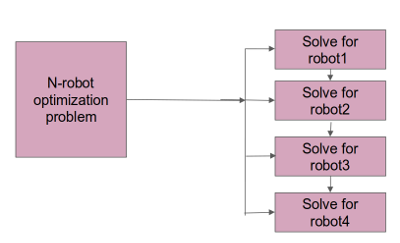
\includegraphics[scale=0.5]{figures/intro/sequential-planning-pipeline.png}
    \caption[Sequential Planning Pipeline for Multi-Robot Systems]{For sequential optimization, an implicit ordering is maintained among the robots, and each robot uses the trajectories of other robots computed before it to compute the collision avoidance constraints while planning its own path. }
    \label{fig:intro_sequential_optimization}
\end{figure}

    For joint optimization, the system-wide trajectory planning is performed simultaneously as a single large-optimization problem returning trajectories for all the robots in one go. The optimization is performed over the larger feasible solution space, involving trajectory variables for all the robots together. 
    \item \textit{Distributed Optimization}, where the trajectory planning problem of each robot is completely decoupled from the other robots. Each robot makes predictions about the others' trajectories based on a prediction model to compute collision-free paths. That is, for an $n$-robot system, each robot considers $n-1$ collision constraints with other robots while planning its trajectory. The per-robot optimization problem becomes simpler to solve and this is repeated over all $n$ robots.
\end{itemize}

Centralized optimization approaches, whether sequential or joint, discussed in \cite{chen2015decoupled}, \cite{incremental_scp_how}, fail to scale efficiently with an increase in the number of robots in the system. The pairwise collision avoidance constraints among the robots scale quadratically with the number of robots. Distributed approaches, on the other hand, are fast to compute paths but susceptible to digressions between the trajectory predictions and actual robot trajectories and have been shown in \cite{dmpc_carlos} to be less effective in collision avoidance. 

To achieve our goal discussed in \ref{intro:multi-robot_aim} of real-time trajectory planning for multiple robots, we choose the distributed optimization paradigm owing to its speed. We aim to achieve computational acceleration on the following two fronts:

\begin{enumerate}
    \item \label{motivation: per_robot} Speeding up the per-robot trajectory optimization 
    \item \label{motivation:parallelization} Avoiding having to loop over all robots while computing individual paths by parallelizing decoupled trajectory computations.
\end{enumerate}

To achieve \ref{motivation: per_robot}, we approximate the trajectory optimization problem as a sequence of matrix operations so that effectively we only need to solve a set of linear equations to obtain the trajectory of each robot. We then vectorize our computations and solve the planning problem for all robots by stacking up independent per-robot problems into a large block matrix. This removes the need to loop over an increasing number of robots and returns trajectories for all robots in a single shot. We cache computationally expensive operations such as block matrix inversing through clever mathematical reformulations of the optimization problem and leverage GPUs to accelerate matrix multiplications. We also compare our approach against a diverse range of state-of-the-art multi-robot path planners and achieve a 2x computational acceleration while not compromising on other metrics such as collisions and trajectory length, as will be shown in Section \ref{sec: GPU_mat_Results}.

\subsection{Stochastic Trajectory Optimization for Robot Manipulators}


Path planning for robot manipulators involves planning a sequence of controls to achieve a desired objective, for example, pushing an object from one point to another or picking and placing an object at a target location. Stochastic Trajectory Optimization is an optimization technique used to generate optimal trajectories for robot manipulators. The STO algorithm optimizes the control inputs of a robot to minimize a cost function that captures the desired task objectives using a probabilistic approach.
It generates a large number of random trajectories and evaluates their cost function values. It then selects the best-performing trajectories and generates new random trajectories around them to further explore the search space. This process is repeated until a satisfactory solution is found.

The STO algorithm is particularly useful for manipulator path planning since it can work with high-dimensional motion spaces and non-differentiable and discontinuous cost functions, It is also robust to uncertainties and disturbances in the environment and sensor noise, which gives it advantages in complex and uncertain planning tasks over gradient-based optimizers. 

In chapter \ref{ch:bl_arm}, we use a version of STO to plan collision-free trajectories for robot manipulators in both the joint-angle space and the Cartesian end-effector space. We design a novel cost function, incorporating collision penalty, joint limit cost, and trajectory length. We then combine our STO planner with a low-level controller for non-prehensile tasks, such as pushing an object on a tabletop from a start position to a desired goal position. 



\section{Thesis Layout}

\begin{itemize}
    \item[C1] This is the introductory chapter, which discusses the scope of the work carried out in this thesis in terms of global and local path planning, addresses the research problems we are tackling and outlines the motivation behind some of the methods we have adopted to solve them.
    \item[C2] In this chapter, we present a background of standard algorithms used for continuous-time and discrete-time trajectory optimization for individual robots that form a necessary prerequisite to understand the ideas discussed in the following chapters. We also discuss two primary paradigms in trajectory optimization - gradient-based optimization and sampling-based optimization, and compare their applications in complex robot systems.
    \item[C3] We present the first contribution of this thesis - Fast Joint Multi-Robot Trajectory Optimization by GPU Accelerated Batch Solution of Distributed Sub-Problems. This algorithm employs mathematical reformulations to allow efficient caching of gradients and convex approximations for collision constraints in multi-robot systems and computes trajectories in near real-time for as many as 36 robots.
    \item[C4] This chapter presents the second contribution of this thesis - a sampling-based trajectory optimization framework for global path planning and its application in designing a bi-level push planner for robot manipulators. We test and show the efficacy of our optimizer in complex tabletop rearrangement scenarios for a few common robot manipulators.
    \item[C5] We conclude with a summary of methods and results discussed in this thesis and the scope of extension of this work in the future.
\end{itemize}
